%% bare_jrnl.tex
%% V1.4b
%% 2015/08/26
%% by Michael Shell
%% see http://www.michaelshell.org/
%% for current contact information.
%%
%% This is a skeleton file demonstrating the use of IEEEtran.cls
%% (requires IEEEtran.cls version 1.8b or later) with an IEEE
%% journal paper.
%%
%% Support sites:
%% http://www.michaelshell.org/tex/ieeetran/
%% http://www.ctan.org/pkg/ieeetran
%% and
%% http://www.ieee.org/

%%*************************************************************************
%% Legal Notice:
%% This code is offered as-is without any warranty either expressed or
%% implied; without even the implied warranty of MERCHANTABILITY or
%% FITNESS FOR A PARTICULAR PURPOSE! 
%% User assumes all risk.
%% In no event shall the IEEE or any contributor to this code be liable for
%% any damages or losses, including, but not limited to, incidental,
%% consequential, or any other damages, resulting from the use or misuse
%% of any information contained here.
%%
%% All comments are the opinions of their respective authors and are not
%% necessarily endorsed by the IEEE.
%%
%% This work is distributed under the LaTeX Project Public License (LPPL)
%% ( http://www.latex-project.org/ ) version 1.3, and may be freely used,
%% distributed and modified. A copy of the LPPL, version 1.3, is included
%% in the base LaTeX documentation of all distributions of LaTeX released
%% 2003/12/01 or later.
%% Retain all contribution notices and credits.
%% ** Modified files should be clearly indicated as such, including  **
%% ** renaming them and changing author support contact information. **
%%*************************************************************************


% *** Authors should verify (and, if needed, correct) their LaTeX system  ***
% *** with the testflow diagnostic prior to trusting their LaTeX platform ***
% *** with production work. The IEEE's font choices and paper sizes can   ***
% *** trigger bugs that do not appear when using other class files.       ***                          ***
% The testflow support page is at:
% http://www.michaelshell.org/tex/testflow/



\documentclass[journal]{IEEEtran}
%
% If IEEEtran.cls has not been installed into the LaTeX system files,
% manually specify the path to it like:
% \documentclass[journal]{../sty/IEEEtran}

%**** LANGUAGE PACKAGES *****
\usepackage[spanish, shorthands=off]{babel}



% Some very useful LaTeX packages include:
% (uncomment the ones you want to load)


% *** MISC UTILITY PACKAGES ***
%
%\usepackage{ifpdf}
% Heiko Oberdiek's ifpdf.sty is very useful if you need conditional
% compilation based on whether the output is pdf or dvi.
% usage:
% \ifpdf
%   % pdf code
% \else
%   % dvi code
% \fi
% The latest version of ifpdf.sty can be obtained from:
% http://www.ctan.org/pkg/ifpdf
% Also, note that IEEEtran.cls V1.7 and later provides a builtin
% \ifCLASSINFOpdf conditional that works the same way.
% When switching from latex to pdflatex and vice-versa, the compiler may
% have to be run twice to clear warning/error messages.



% *** CITATION PACKAGES ***
%
\usepackage{cite}
% cite.sty was written by Donald Arseneau
% V1.6 and later of IEEEtran pre-defines the format of the cite.sty package
% \cite{} output to follow that of the IEEE. Loading the cite package will
% result in citation numbers being automatically sorted and properly
% "compressed/ranged". e.g., [1], [9], [2], [7], [5], [6] without using
% cite.sty will become [1], [2], [5]--[7], [9] using cite.sty. cite.sty's
% \cite will automatically add leading space, if needed. Use cite.sty's
% noadjust option (cite.sty V3.8 and later) if you want to turn this off
% such as if a citation ever needs to be enclosed in parenthesis.
% cite.sty is already installed on most LaTeX systems. Be sure and use
% version 5.0 (2009-03-20) and later if using hyperref.sty.
% The latest version can be obtained at:
% http://www.ctan.org/pkg/cite
% The documentation is contained in the cite.sty file itself.


% *** GRAPHICS RELATED PACKAGES ***
%
\ifCLASSINFOpdf
 \usepackage[pdftex]{graphicx}
 \usepackage{subfigure} % subfiguras
  % declare the path(s) where your graphic files are 
 \graphicspath{ {images/} }
  % and their extensions so you won't have to specify these with
  % every instance of \includegraphics
  \DeclareGraphicsExtensions{.pdf,.jpeg,.png}
\else
  % or other class option (dvipsone, dvipdf, if not using dvips). graphicx
  % will default to the driver specified in the system graphics.cfg if no
  % driver is specified.
  % \usepackage[dvips]{graphicx}
  % declare the path(s) where your graphic files are
  % \graphicspath{{../eps/}}
  % and their extensions so you won't have to specify these with
  % every instance of \includegraphics
  % \DeclareGraphicsExtensions{.eps}
\fi
% graphicx was written by David Carlisle and Sebastian Rahtz. It is
% required if you want graphics, photos, etc. graphicx.sty is already
% installed on most LaTeX systems. The latest version and documentation
% can be obtained at: 
% http://www.ctan.org/pkg/graphicx
% Another good source of documentation is "Using Imported Graphics in
% LaTeX2e" by Keith Reckdahl which can be found at:
% http://www.ctan.org/pkg/epslatex
%
% latex, and pdflatex in dvi mode, support graphics in encapsulated
% postscript (.eps) format. pdflatex in pdf mode supports graphics
% in .pdf, .jpeg, .png and .mps (metapost) formats. Users should ensure
% that all non-photo figures use a vector format (.eps, .pdf, .mps) and
% not a bitmapped formats (.jpeg, .png). The IEEE frowns on bitmapped formats
% which can result in "jaggedy"/blurry rendering of lines and letters as
% well as large increases in file sizes.
%
% You can find documentation about the pdfTeX application at:
% http://www.tug.org/applications/pdftex





% *** MATH PACKAGES ***
%
\usepackage{amsmath}
% A popular package from the American Mathematical Society that provides
% many useful and powerful commands for dealing with mathematics.
%
% Note that the amsmath package sets \interdisplaylinepenalty to 10000
% thus preventing page breaks from occurring within multiline equations. Use:
%\interdisplaylinepenalty=2500
% after loading amsmath to restore such page breaks as IEEEtran.cls normally
% does. amsmath.sty is already installed on most LaTeX systems. The latest
% version and documentation can be obtained at:
% http://www.ctan.org/pkg/amsmath





% *** SPECIALIZED LIST PACKAGES ***
%
\usepackage{algorithmic}
% algorithmic.sty was written by Peter Williams and Rogerio Brito.
% This package provides an algorithmic environment fo describing algorithms.
% You can use the algorithmic environment in-text or within a figure
% environment to provide for a floating algorithm. Do NOT use the algorithm
% floating environment provided by algorithm.sty (by the same authors) or
% algorithm2e.sty (by Christophe Fiorio) as the IEEE does not use dedicated
% algorithm float types and packages that provide these will not provide
% correct IEEE style captions. The latest version and documentation of
% algorithmic.sty can be obtained at:
% http://www.ctan.org/pkg/algorithms
% Also of interest may be the (relatively newer and more customizable)
% algorithmicx.sty package by Szasz Janos:
% http://www.ctan.org/pkg/algorithmicx



\usepackage{xspace} 

% *** ALIGNMENT PACKAGES ***
%
\usepackage{array}
% Frank Mittelbach's and David Carlisle's array.sty patches and improves
% the standard LaTeX2e array and tabular environments to provide better
% appearance and additional user controls. As the default LaTeX2e table
% generation code is lacking to the point of almost being broken with
% respect to the quality of the end results, all users are strongly
% advised to use an enhanced (at the very least that provided by array.sty)
% set of table tools. array.sty is already installed on most systems. The
% latest version and documentation can be obtained at:
% http://www.ctan.org/pkg/array


% IEEEtran contains the IEEEeqnarray family of commands that can be used to
% generate multiline equations as well as matrices, tables, etc., of high
% quality.




% *** SUBFIGURE PACKAGES ***
%\ifCLASSOPTIONcompsoc
%  \usepackage[caption=false,font=normalsize,labelfont=sf,textfont=sf]{subfig}
%\else
%  \usepackage[caption=false,font=footnotesize]{subfig}
%\fi
% subfig.sty, written by Steven Douglas Cochran, is the modern replacement
% for subfigure.sty, the latter of which is no longer maintained and is
% incompatible with some LaTeX packages including fixltx2e. However,
% subfig.sty requires and automatically loads Axel Sommerfeldt's caption.sty
% which will override IEEEtran.cls' handling of captions and this will result
% in non-IEEE style figure/table captions. To prevent this problem, be sure
% and invoke subfig.sty's "caption=false" package option (available since
% subfig.sty version 1.3, 2005/06/28) as this is will preserve IEEEtran.cls
% handling of captions.
% Note that the Computer Society format requires a larger sans serif font
% than the serif footnote size font used in traditional IEEE formatting
% and thus the need to invoke different subfig.sty package options depending
% on whether compsoc mode has been enabled.
%
% The latest version and documentation of subfig.sty can be obtained at:
% http://www.ctan.org/pkg/subfig




% *** FLOAT PACKAGES ***
%
%\usepackage{fixltx2e}
% fixltx2e, the successor to the earlier fix2col.sty, was written by
% Frank Mittelbach and David Carlisle. This package corrects a few problems
% in the LaTeX2e kernel, the most notable of which is that in current
% LaTeX2e releases, the ordering of single and double column floats is not
% guaranteed to be preserved. Thus, an unpatched LaTeX2e can allow a
% single column figure to be placed prior to an earlier double column
% figure.
% Be aware that LaTeX2e kernels dated 2015 and later have fixltx2e.sty's
% corrections already built into the system in which case a warning will
% be issued if an attempt is made to load fixltx2e.sty as it is no longer
% needed.
% The latest version and documentation can be found at:
% http://www.ctan.org/pkg/fixltx2e


%\usepackage{stfloats}
% stfloats.sty was written by Sigitas Tolusis. This package gives LaTeX2e
% the ability to do double column floats at the bottom of the page as well
% as the top. (e.g., "\begin{figure*}[!b]" is not normally possible in
% LaTeX2e). It also provides a command:
%\fnbelowfloat
% to enable the placement of footnotes below bottom floats (the standard
% LaTeX2e kernel puts them above bottom floats). This is an invasive package
% which rewrites many portions of the LaTeX2e float routines. It may not work
% with other packages that modify the LaTeX2e float routines. The latest
% version and documentation can be obtained at:
% http://www.ctan.org/pkg/stfloats
% Do not use the stfloats baselinefloat ability as the IEEE does not allow
% \baselineskip to stretch. Authors submitting work to the IEEE should note
% that the IEEE rarely uses double column equations and that authors should try
% to avoid such use. Do not be tempted to use the cuted.sty or midfloat.sty
% packages (also by Sigitas Tolusis) as the IEEE does not format its papers in
% such ways.
% Do not attempt to use stfloats with fixltx2e as they are incompatible.
% Instead, use Morten Hogholm'a dblfloatfix which combines the features
% of both fixltx2e and stfloats:
%
% \usepackage{dblfloatfix}
% The latest version can be found at:
% http://www.ctan.org/pkg/dblfloatfix




%\ifCLASSOPTIONcaptionsoff
%  \usepackage[nomarkers]{endfloat}
% \let\MYoriglatexcaption\caption
% \renewcommand{\caption}[2][\relax]{\MYoriglatexcaption[#2]{#2}}
%\fi
% endfloat.sty was written by James Darrell McCauley, Jeff Goldberg and 
% Axel Sommerfeldt. This package may be useful when used in conjunction with 
% IEEEtran.cls'  captionsoff option. Some IEEE journals/societies require that
% submissions have lists of figures/tables at the end of the paper and that
% figures/tables without any captions are placed on a page by themselves at
% the end of the document. If needed, the draftcls IEEEtran class option or
% \CLASSINPUTbaselinestretch interface can be used to increase the line
% spacing as well. Be sure and use the nomarkers option of endfloat to
% prevent endfloat from "marking" where the figures would have been placed
% in the text. The two hack lines of code above are a slight modification of
% that suggested by in the endfloat docs (section 8.4.1) to ensure that
% the full captions always appear in the list of figures/tables - even if
% the user used the short optional argument of \caption[]{}.
% IEEE papers do not typically make use of \caption[]'s optional argument,
% so this should not be an issue. A similar trick can be used to disable
% captions of packages such as subfig.sty that lack options to turn off
% the subcaptions:
% For subfig.sty:
% \let\MYorigsubfloat\subfloat
% \renewcommand{\subfloat}[2][\relax]{\MYorigsubfloat[]{#2}}
% However, the above trick will not work if both optional arguments of
% the \subfloat command are used. Furthermore, there needs to be a
% description of each subfigure *somewhere* and endfloat does not add
% subfigure captions to its list of figures. Thus, the best approach is to
% avoid the use of subfigure captions (many IEEE journals avoid them anyway)
% and instead reference/explain all the subfigures within the main caption.
% The latest version of endfloat.sty and its documentation can obtained at:
% http://www.ctan.org/pkg/endfloat
%
% The IEEEtran \ifCLASSOPTIONcaptionsoff conditional can also be used
% later in the document, say, to conditionally put the References on a 
% page by themselves.




% *** PDF, URL AND HYPERLINK PACKAGES ***
%
%\usepackage{url}
% url.sty was written by Donald Arseneau. It provides better support for
% handling and breaking URLs. url.sty is already installed on most LaTeX
% systems. The latest version and documentation can be obtained at:
% http://www.ctan.org/pkg/url
% Basically, \url{my_url_here}.


\usepackage{authblk}

% *** Do not adjust lengths that control margins, column widths, etc. ***
% *** Do not use packages that alter fonts (such as pslatex).         ***
% There should be no need to do such things with IEEEtran.cls V1.6 and later.
% (Unless specifically asked to do so by the journal or conference you plan
% to submit to, of course. )


% correct bad hyphenation here
\hyphenation{op-tical net-works semi-conduc-tor}

% Paquete para saltos del inea
\usepackage[utf8]{inputenc}
\usepackage[table,xcdraw]{xcolor}

% Paquete para utilizar colores
\usepackage{color}



\begin{document}
%
% paper title
% Titles are generally capitalized except for words such as a, an, and, as,
% at, but, by, for, in, nor, of, on, or, the, to and up, which are usually
% not capitalized unless they are the first or last word of the title.
% Linebreaks \\ can be used within to get better formatting as desired.
% Do not put math or special symbols in the title.
\title{ Tiers: Sistema de clasificación de fiabilidad para Data Centers }
%
%
% author names and IEEE memberships
% note positions of commas and nonbreaking spaces ( ~ ) LaTeX will not break
% a structure at a ~ so this keeps an author's name from being broken across
% two lines.
% use \thanks{} to gain access to the first footnote area
% a separate \thanks must be used for each paragraph as LaTeX2e's \thanks
% was not built to handle multiple paragraphs
%

\author{Manuel Figueroa,\IEEEmembership{ Estudiante, ITCR}}% <-this % stops a space
\affil[]{\textit{MC-6006 Redes de Computadores Avanzadas}}
\affil[]{\textit{Instituto Tecnológico de Costa Rica}}
\affil[]{\textit{mfigueroacr@gmail.com}}

% note the % following the last \IEEEmembership and also \thanks - 
% these prevent an unwanted space from occurring between the last author name
% and the end of the author line. i.e., if you had this:
% 
% \author{....lastname \thanks{...} \thanks{...} }
%                     ^------------^------------^----Do not want these spaces!
%
% a space would be appended to the last name and could cause every name on that
% line to be shifted left slightly. This is one of those "LaTeX things". For
% instance, "\textbf{A} \textbf{B}" will typeset as "A B" not "AB". To get
% "AB" then you have to do: "\textbf{A}\textbf{B}"
% \thanks is no different in this regard, so shield the last } of each \thanks
% that ends a line with a % and do not let a space in before the next \thanks.
% Spaces after \IEEEmembership other than the last one are OK (and needed) as
% you are supposed to have spaces between the names. For what it is worth,
% this is a minor point as most people would not even notice if the said evil
% space somehow managed to creep in.



% The paper headers
\markboth{Redes investigación 1: TIERS en Data Centers , Agosto 2020}%
{Shell \MakeLowercase{\textit{et al.}}: Tiers: Sistema de clasificación de fiabilidad para Data Centers }
% The only time the second header will appear is for the odd numbered pages
% after the title page when using the twoside option.
% 
% *** Note that you probably will NOT want to include the author's ***
% *** name in the headers of peer review papers.                   ***
% You can use \ifCLASSOPTIONpeerreview for conditional compilation here if
% you desire.




% If you want to put a publisher's ID mark on the page you can do it like
% this:
%\IEEEpubid{0000--0000/00\$00.00~\copyright~2015 IEEE}
% Remember, if you use this you must call \IEEEpubidadjcol in the second
% column for its text to clear the IEEEpubid mark.



% use for special paper notices
%\IEEEspecialpapernotice{(Invited Paper)}




% make the title area
\maketitle

% As a general rule, do not put math, special symbols or citations
% in the abstract or keywords.
\begin{abstract}
  Investigación acerca del estándar de clasificación del Uptime Institute acerca de la fiabilidad
  de los centros de datos y cuales criterios se utilian para categorizarlos.
  Se investiga además de la definición correspondiente a cada una de las categorías, la situación de
  los data centers más empleados en la industría así como algunos data centers existentes en el país.
\end{abstract}

% Note that keywords are not normally used for peerreview papers.
\begin{IEEEkeywords}
TIERS, Data Center, Redes de Computadores Avanzadas
\end{IEEEkeywords}



% For peer review papers, you can put extra information on the cover
% page as needed:
% \ifCLASSOPTIONpeerreview
% \begin{center} \bfseries EDICS Category: 3-BBND \end{center}
% \fi
%
% For peerreview papers, this IEEEtran command inserts a page break and
% creates the second title. It will be ignored for other modes.
\IEEEpeerreviewmaketitle




% The very first letter is a 2 line initial drop letter followed
% by the rest of the first word in caps.
% 
% form to use if the first word consists of a single letter:
% \IEEEPARstart{A}{demo} file is ....
% 
% form to use if you need the single drop letter followed by
% normal text (unknown if ever used by the IEEE):
% \IEEEPARstart{A}{}demo file is ....
% 
% Some journals put the first two words in caps:
% \IEEEPARstart{T}{his demo} file is ....
% 
% Here we have the typical use of a "T" for an initial drop letter
% and "HIS" in caps to complete the first word.

%\IEEEtriggercmd{\enlargethispage{-5in}}
\section{Introduccióm}
\IEEEPARstart{La} industria de los centros de datos ha utilizado la clasificación por niveles \emph{TIER} presentada
por el Uptime Institute como un mecanismo para categorizar las configuraciones y 
requirimientos de un \emph{Data Center}. \cite{arno_friedl_gross_schuerger_2012,pitt_turner}.
Tanto el \emph{Uptime Institute}, como el \emph{Telecommunications Industry Association} con su estándar \textbf{TIA-942}\cite{TIA}, clasifican los 
data center en cuatro categorias dependiendo de aspectos relacionados a la fiabilidad, disponibilidad, confiabilidad y durabilidad.
Según el Uptime institute, los primeros TIER I aparecen a inicio de la decada de 1960, Tier II en los 70, y Tier III a finales de los años 80 y principios de los 90, y finalmente
se incorpora la definición de Tier IV en 1994 con la disponibilidad de equipos con doble fuente de poder.

\section{Data Centers}
Un Data Center, es un lugar físico que alberga los sistemas críticos que sustentan una red computacional de una o varias organizaciones, se caracterizan por tener gran cantidad de equipo informático 
de gestión de energía y sistemas de enfriamiento y seguridad para velar por la continuidad del servicio brindado en las organizaciones.
Un banco o una entidad gubernamental requiere de los servicios de un data center para gestionar toda la información y transacciones asociadas a su respectiva finalidad. De igual manera empresas privadas pueden hacer
uso de estos data center para gestionar y administrar sus transacciones, comunicaciones e información.

Algunos de los centros de datos se construyen también con la finalidad de soportar la operación de clientes externos, es decir se alquila su poder computacional y de almacenamiento para que sea utilizado por
clientes mediante un servicio de subscripción \cite{amazon_2003}.

\section{Servicios de un Data Center}
Segun CISCO \cite{cisco_2020}, los data center son comúnmente utilizados por las organizaciones y empresas principalmente para soportar aplicaciones y actividades necesarias para su operación tales
como:
\begin{itemize}
  \item Email y archivos compartidos.
  \item Aplicaciones de productividad (Git, TFS, Jira).
  \item Sistemas de planeamiento empresarial (ERP) y bases de datos.
  \item Big data, sistemas de inteligencia artificial y machine learning,
  \item Virtual desktops, comunicaciones y servicios de colaboración.
\end{itemize}

\section{Componentes de un Data Center}
Además de la infraestructura física, sistemas de enfriamiento y de gestión eléctrica, un data center se compone principalmente de equipo de compúto tal como:
router, switches, firewalls, sistemas de almacenamiento y servidores.
Todos estos componentes se utilizan para proveer los principales servicios del data center que se pueden categorizar en:
\begin{itemize}
  \item Infraestructura de Red: Conectividad entre servidores, servicios, y sistemas de almacenamiento.
  \item Infraestructura de Almacenamiento: La finalidad de un data center son los datos, por lo que el almacenamiento constituye uno de sus valores primarios.
  \item Recursos computacionales: Los data center proveen el poder computacional para ejecutar las aplicaciones que requiere una organización, cuentan con suficiente poder de procesamiento, memoria y almacenamiento para que 
  los servicios que proveen estas aplicaciones sean accesibles a los usuarios que lo requieran.
\end{itemize}
Según el estándar TIA-942 un DataCenter debe componerse de los subsistemas:
\begin{itemize}
  \item Telecomunicaciones.
  \item Arquitectura.
  \item Sistema eléctrico
  \item Sistema mecánico.
\end{itemize}

\subsection{Telecomunicaciones}
\subsection{Arquitectura}
\subsection{Sistema eléctrico}
\subsection{Sistema mecánico}
\section{Definición de los Tiers}
Las distintas clasificaciones Tier indican un nivel de fiabilidad aceptada para un data center, categorizada en los cuatro
niveles mencionados anteriormente. Esta fiabilidad esta asociada a un nivel esperao de disponibilidad y tolerancia a fallas, por lo que el costo
mantener una infraestructura con mayor disponibilidad es mucho mayor.

El estándar define cuatro categorias, ordenadas de menor a mayor rango de disponibilidad, asi que entre más alto sea el Tier del data center
este tendrá un mejor servicio con respecto a la tolerancia a fallos en general. 
En la figura \ref{volico} se detalla la principal diferencia con respecto al tiempo de disponibilidad relativo de cada categoría del sistema de clasificación TIER.
\begin{figure*}
  \centering
  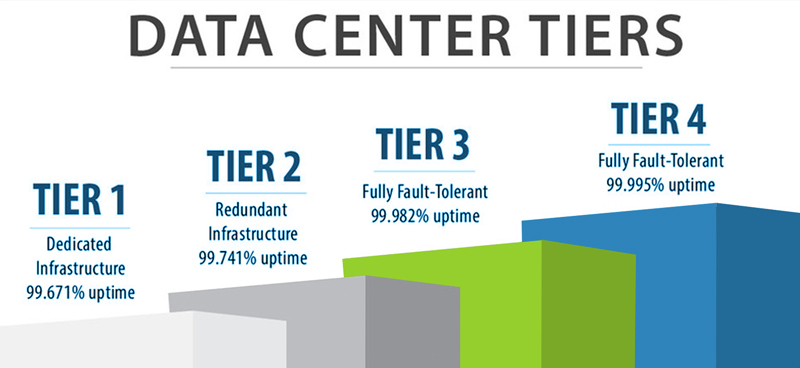
\includegraphics[scale=0.3]{Data-Center-Tiers.jpg}
  \caption{Diferencias de disponibilidad entre clasificaciones TIER, tomado de \cite{volico_2018}}
  \label{volico}
\end{figure*}
\subsection{Tier I}
Según la definición del estándar en \cite{pitt_turner}, un data center Tier I es susceptible a interrupciones en el servicio por parte de actividades  planeadas y no planeadas.
Posee distribución del poder de computación y un sistema de enfriamiento, pero puede carecer de un piso elevado y sistemas de protección ante fallas 
eléctricas como una UPS o un generador y si se tuviesen son módulos individuales, por lo que son potencialmente muchos puntos de falla.
Parte de la definición del Tier I es que toda su infraestructura debe apagarse completamente de manera anual para realizar mantenimiento preventivo y trabajos de reparación.
Cuando se presentan situaciones urgentes, son susceptibles a más interrupciones en el servicio, asi  como cuando ocurren fallas espontáneas en equipos que pueden causar una caída total del servicio brindado por el data center.
\subsection{Distribucion de Energía para Tier I}
Tier I se compone de una única fuente de distribución de energía y de enfriamiento, sin componentes redundantes que proveen un 99.671\% de disponibilidad\cite{pitt_turner}.
Este porcentaje de disponibilidad se puede traducir en alrededor de 29 horas de impacto en el servicio al año.
\subsection{Tier II}
En el segundo nivel del estándar del Uptime Institute, se encuentran los Tier II con componentes redundantes, que los hacen ligeramente menos susceptibles a interrupciones inesperadas en el servicio.
Tienen que construirse en un piso elevado, contar con dispositivos para mitigar fallas en el sistema eléctrico (UPS y generadores). Sin embargo, cuentan con una única vía para la distribución de energía,
por lo que un mantenimiento del mecanismo de distribución de energía require un tiempo de baja total del sistema.
\subsection{Distribución de Energía para Tier II}
Tier II se compone de una vía única para la distribución de energía y enfriamiento, con componentes redundantes por lo que ofrece una disponibilidad relativa de 99.741\% del tiempo. Esto es equivalente a 
que el servicio no se encuentra inactivo por más de 22 horas al año.
\subsection{Tier III}
El tercer nivel del estándar se enfoca en mantenimientos simultáneos, es decir que permiten realizar actividades planeadas sobre la infraestructura del data center sin interrumpir la prestación de servicios.
Entre las actividades planeadas se incluyen mantenimiento preventivo y reparación o sustitución de equipos y componentes, así como la capacidad de agregar o remover parte de estos para aumentar o disminuir la capacidad
del data center. 
Las actividades no planeadas como errores o fallas espontáneas de los componentes aún causarían una interrupción en el servicio. La manera más común de verificar si se encuentra ante un Tier III es la capacidad de realizar cualquier
trabajo planeado sin interrupciones al servicio que brinda el data center.
\subsection{Distribución de Energía para Tier III}
Tier III se compone de varias fuentes distintas para la distribución de la energía y el sistema de enfriamiento, sin embargo solo una se encuentra activa a la vez. Los Tier III además cuentan con componentes redundantes que permiten
un manteniento concurrente, estos data centers ofrecen una disponibilidad de 99.982\%. En este nivel el porcentaje de disponibilidad equivale a tan solo 1.6 horas de baja en el servicio de manera anual.
\subsection{Tier IV}
En este nivel se considera al data center como tolerante a fallas, los data center de tipo Tier IV proveen las capacidades de infraestructura que permiten realizar cualquier actividad planeada sin afectación al servicio 
brindado. Se cuenta con vías de distribución de energía y enfriamiento simultaneamente activas, lo que significa que cada equipo cuenta con almenos dos UPS separadas, además los equipos cuentan con doble entrada de energía.
\subsection{Distribución de Energía para Tier IV}
Se componen de múltiples vías para la distribución de energía y enfriamiento que se encuentran activas de manera simúltanea, esta configuración permite un 99,9995\% de disponibilidad. Los data centers tipo Tier IV solamente presentan bajas en el servicio a lo sumo 0.5 horas cada año.
\section{Proceso de Certificación TIER}
En \cite{george}, se detalla el sistema de certificación definido por el Uptime Institute como única entidad encargada de calificar y certificar los diseños de instalaciones destinadas a data centers. 
Se consideran aspectos relevantes de la infraestructura y topología para garantizar la ausencia de puntos débiles en las infraestructuras de los centros de datos.
Entre los pasos seguidos para obtener la certificación necesaria están:
\\
\\
\begin{itemize}
  \item Tier Gap Analysis que permite identificar problemas que impidan cumplir los objetivos de Tier.
  \item Una revisión completa de los documentos de diseño del data center.
  \item Verificación en sitio de la infraestructura instalada.
  \item Evaluación de la presencia y eficacia de la administración y las operaciones del data center.
\end{itemize}
\section{Data Centers más utilizados}
Según \cite{amazon_2003}, uno de los data centers más utilizados en el mundo es el de amazon.com que provee mediante su plataforma de servicios AWS este se encuentra bajo la modalidad Tier IV
lo que permite a sus usuarios alcanzar un alto nivel de disponibilidad de los servicios alojados en su plataforma.
De igual manera, según Hu et al.\cite{zhengbing_gnatyuk_koval_gnatyuk_bondarovets_2017} muchos otros data centers disponibles para su uso público mediante un servicio de subscripción como los ofrecidos por Microsoft son también Tier IV.
\section{Situación en Costa Rica}
En Costa Rica existen al menos 14 data centers certificados por el Uptime Institute. De los cuales los correspondientes al INS (\emph{Instituto Nacional de Seguros}) y al Ministerio de Hacienda cuentan con la certificación Tier IV \cite{castro}.
también otras instituciones gubernamentales como RECOPE y privadas como CODISA y ADN cuentan con centros de datos del Tipo Tier III. En la tabla \ref{tablacr} se presenta un resumen de los data center certificados en Costa Rica.

% Please add the following required packages to your document preamble:
% \usepackage[table,xcdraw]{xcolor}
% If you use beamer only pass "xcolor=table" option, i.e. \documentclass[xcolor=table]{beamer}
\begin{table}[]
  \begin{tabular}{|l|l|}
  \hline
  \rowcolor[HTML]{DAE8FC} 
  {\color[HTML]{00009B} Data Center}                                                                                                                     & {\color[HTML]{00009B} Tier} \\ \hline
  Ins, Hacienda                                                                                                                                          & IV                          \\ \hline
  \begin{tabular}[c]{@{}l@{}}Recope, BCR, Caja de Ande, ADN,Green Data\\ Critical Colocation, Codisa, ICE, Mutual Alajuela,\\ Banco Popular\end{tabular} & III                         \\ \hline
  HP, CAC, Mucap                                                                                                                                         & II                          \\ \hline
  \end{tabular}
  \caption{Data centers certificados en Costa Rica.\cite{castro}} \label{tablacr}
  \end{table}

\section{Conclusiones}
El sistema de clasificación del Uptime Institute es un mecanismo útil para conocer la fiabilidad de un data center de manera agnóstica a
los proveedores de los servicios y de los equipos en general.
Las medidas de disponibilidad y fiabilidad se basan en las caracteristicas de los equipos y en la infraestructura que compone al data center asi como a la presencia o ausencia
de sistemas de gestión de energía, enfriamiento y seguridad.

Un data center certificado con la norma Tier permite de antemano conocer su tiempo esperado de disponibilidad y saber el riesgo que corren los servicios a no estar disponibles 
en un tiempo determinado.

Debido a la creciente expansión en los servicios basados en la conectividad y comunicación, así como al auge de tópicos como el internet de las cosas y las tecnologías móviles 
se tiene una necesidad creciente en el acceso a recursos computacionales no solo de alto rendimiento, si no que con una alta disponibilidad, por lo que servicios alojados en data centers
de acceso público son una opción importante para poder lograr continuidad en los servicios sin la inversión requerida para una infraestructura local con el mismo nivel de disponibilidad.

Los servicios brindados por grandes empresas como Amazon ofrecen la disponibilidad y seguridad de un data center Tier IV o incluso ligeramente superior, en términos del porcentaje de disponibilidad, a un 
costo rasonable para las organizaciones.

De igual manera aquellas organizaciones que por la sensibilidad de sus datos requieran una infraestructura propia, pueden utilizar las certificaciones Tier como una garantía en el diseños
de sus centros de datos y en la capacidad de respuesta ante fallas o actividades planeadas que no afecten la prestación de sus servicios.

% references section

% can use a bibliography generated by BibTeX as a .bbl file
% BibTeX documentation can be easily obtained at:
% http://mirror.ctan.org/biblio/bibtex/contrib/doc/
% The IEEEtran BibTeX style support page is at:
% http://www.michaelshell.org/tex/ieeetran/bibtex/
\bibliographystyle{IEEEtran}
% argument is your BibTeX string definitions and bibliography database(s)
\bibliography{bibliography}



% that's all folks
\end{document}


